% questions.tex -- Module 6 (Electromagnetism) short-answer booklet, HSC Section II style.
% 20 questions, 90 marks: Topic 1 Q1-5 (22 marks), Topic 2 Q6-10 (23), Topic 3 Q11-15 (22),
% Marking guidelines and sample answers: answers.tex.
% Every number: checks/m6-short-answer/numbers.py
% Build: TEXINPUTS=.: xelatex questions.tex (twice)
\documentclass[12pt]{article}
\usepackage{quiz}
\hypersetup{pdftitle={Short Answer Questions - Module 6 - Electromagnetism}}

\begin{document}
\quiztitle{Year 12 Physics}{Short Answer Questions - Module 6 - Electromagnetism}
\begin{center}
  20 questions \textperiodcentered\ 90 marks \textperiodcentered\ allow about 2 hours 40 minutes\\[2pt]
  Show all working. Use $e = \qty{1.602e-19}{C}$, $m_\mathrm{e} = \qty{9.109e-31}{kg}$,
  $m_\mathrm{p} = \qty{1.673e-27}{kg}$, $\mu_0 = 4\pi \times 10^{-7}\,\si{N.A^{-2}}$,
  $g = \qty{9.8}{m.s^{-2}}$.\\
  {\small $\times$ = magnetic field into the page \qquad $\bullet$ = magnetic field out of the page}
\end{center}

% =====================================================================
\firsttopictitle{Topic 1 - Charged Particles in Electric and Magnetic Fields}

% ---- Q1 (electron accelerated between plates)
\begin{saq}{4}
Two parallel plates are \qty{4.0}{cm} apart, with a potential difference of \qty{500}{V} between them.
An electron starts from rest at the negative plate.
\qpartL{a}{1}{Calculate the electric field strength between the plates.}{2}
\qpartL{b}{1}{Calculate the acceleration of the electron.}{3}
\qpartL{c}{2}{Calculate the speed of the electron when it reaches the positive plate.}{4}
\end{saq}

% ---- Q2 (electron deflected between plates)
\Needspace{34\baselineskip}
\begin{saq}{5}
An electron enters the space between two horizontal parallel plates at \qty{2.0e7}{m.s^{-1}}, moving
parallel to the plates, halfway between them. The plates are \qty{6.0}{cm} long and \qty{2.0}{cm} apart.
The top plate is at \qty[retain-explicit-plus]{+150}{V} and the bottom plate is at \qty{0}{V}.
\begin{center}
  \begin{tikzpicture}
    \draw[line width=1.3pt] (1,1.6) -- (6,1.6) node[right, font=\small] {\qty[retain-explicit-plus]{+150}{V}};
    \draw[line width=1.3pt] (1,0) -- (6,0) node[right, font=\small] {\qty{0}{V}};
    \fill (-0.2,0.8) circle (2pt) node[left, font=\small] {$e^-$}; \draw[->, line width=0.7pt] (-0.1,0.8) -- (0.8,0.8) node[above, font=\small] {\qty{2.0e7}{m.s^{-1}}};
    \draw[|<->|, line width=0.4pt] (1,-0.45) -- (6,-0.45) node[midway, below, font=\small] {\qty{6.0}{cm}};
    \draw[|<->|, line width=0.4pt] (7.4,0) -- (7.4,1.6) node[midway, right, font=\small] {\qty{2.0}{cm}};
  \end{tikzpicture}
\end{center}
\qpartL{a}{3}{Calculate the vertical distance the electron moves while it is between the plates.}{8}
\qpartL{b}{2}{Compare the path of the electron between the plates with the path of a projectile in
Earth's gravitational field.}{4}
\end{saq}

% ---- Q3 (proton in a magnetic field)
\Needspace{24\baselineskip}
\begin{saq}{4}
A proton moves at \qty{4.0e6}{m.s^{-1}} at right angles to a uniform magnetic field of \qty{0.25}{T}.
\qpartL{a}{2}{Show that the radius of its circular path is $r = \dfrac{mv}{qB}$.}{5}
\qpartL{b}{1}{Calculate the radius of the proton's path.}{2}
\qpartL{c}{1}{Explain why the kinetic energy of the proton does not change.}{2}
\end{saq}

% ---- Q4 (velocity selector and mass spectrometer)
\Needspace{36\baselineskip}
\begin{saq}{5}
Singly charged positive ions pass through a velocity selector, where a uniform electric field of
\qty{2.0e4}{V.m^{-1}} (directed down the page) is at right angles to a uniform magnetic field of
\qty{0.10}{T} (directed into the page). Ions that pass
straight through then enter a second uniform magnetic field of \qty{0.20}{T}, directed into the page,
where they travel in a semicircle of radius \qty{0.24}{m}.
\begin{center}
  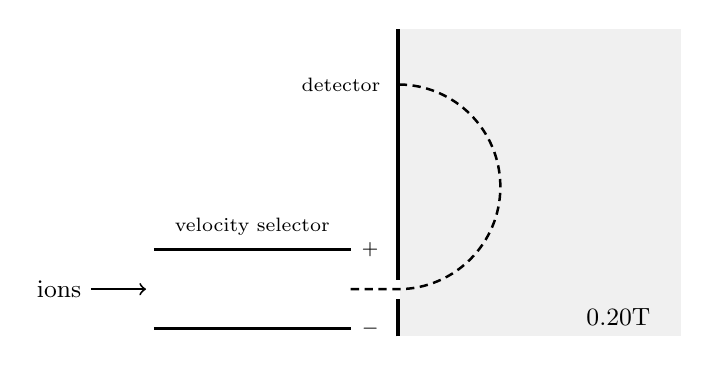
\begin{tikzpicture}
    \draw[line width=1.2pt] (0.5,0.5) -- (3,0.5) node[right, font=\scriptsize] {$+$}; \draw[line width=1.2pt] (0.5,-0.5) -- (3,-0.5) node[right, font=\scriptsize] {$-$};
    \fieldin{0.8}{-0.25}{2.8}{0.25}{0.5}
    \node[font=\scriptsize] at (1.75,0.8) {velocity selector};
    \draw[->, line width=0.7pt] (-0.3,0) -- (0.4,0); \node[left, font=\small] at (-0.3,0) {ions};
    \draw[line width=1.2pt] (3.6,-0.6) -- (3.6,-0.12); \draw[line width=1.2pt] (3.6,0.12) -- (3.6,3.3);
    \fill[black!6] (3.62,-0.6) rectangle (7.2,3.3); \fieldin{3.9}{-0.35}{7.0}{3.1}{0.5}
    \draw[line width=0.9pt, dash pattern=on 3pt off 2pt] (3,0) -- (3.6,0) arc (-90:90:1.3);
    \node[font=\small, fill=black!6] at (6.4,-0.35) {\qty{0.20}{T}};
    \node[left, font=\scriptsize, align=right] at (3.5,2.6) {detector};
  \end{tikzpicture}
\end{center}
\qpartL{a}{2}{Explain why only ions with one particular speed pass straight through the velocity
selector, and calculate this speed.}{5}
\qpartL{b}{2}{Calculate the mass of the ions.}{4}
\qpartL{c}{1}{Heavier ions with the same charge also pass through the velocity selector. Where do they
hit the detector, compared with these ions? Justify your answer.}{2}
\end{saq}

% ---- Q5 (compare E and B fields)
\Needspace{110mm}
\begin{saq}{4}
Compare the motion of a charged particle that enters a uniform electric field at right angles to the
field with the motion of the same particle entering a uniform magnetic field at right angles to the
field.
\alines{10}
\end{saq}

% =====================================================================
\topictitle{Topic 2 - The Motor Effect}

% ---- Q6 (force on a conductor at an angle)
\begin{saq}{4}
A straight wire \qty{0.25}{m} long carries a current of \qty{4.0}{A}. It lies at \ang{50} to a uniform
magnetic field of \qty{0.30}{T}, in the plane of the page.
\begin{center}
  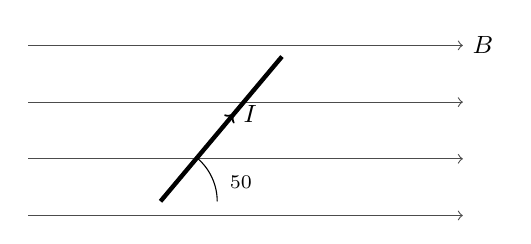
\begin{tikzpicture}[scale=1.2]
    \foreach \y in {0,0.6,...,1.9} \draw[->, line width=0.4pt, black!70] (0,\y) -- (4.6,\y);
    \node[right, font=\small] at (4.6,1.8) {$B$};
    \draw[line width=1.6pt] (1.4,0.15) -- ++(50:2.0);
    \draw[->, line width=0.8pt] (1.85,0.69) -- ++(50:0.5) node[right, font=\small] {$I$};
    \draw (2.0,0.15) arc (0:50:0.6); \node[font=\scriptsize] at (2.25,0.35) {\ang{50}};
  \end{tikzpicture}
\end{center}
\qpartL{a}{2}{Calculate the magnitude of the force on the wire.}{4}
\qpartL{b}{1}{State the direction of the force on the wire.}{2}
\qpartL{c}{1}{How should the wire be placed to experience the greatest possible force?}{2}
\end{saq}

% ---- Q7 (parallel wires; the ampere)
\Needspace{24\baselineskip}
\begin{saq}{5}
Two long parallel wires are \qty{5.0}{cm} apart. They carry currents of \qty{8.0}{A} and \qty{12}{A} in
the same direction.
\qpartL{a}{2}{Calculate the force per metre between the wires.}{4}
\qpartL{b}{1}{State whether the wires attract or repel, and explain why.}{2}
\qpartL{c}{2}{Explain how the force between parallel wires was used (until 2019) to define the
ampere, and how Newton's third law applies to the two wires.}{5}
\end{saq}

% ---- Q8 (practical: force on a wire, balance method)
% Data: l = 0.050 m, B = 0.12 T: extra balance reading = B I l / g (grams per amp = 0.61).
\Needspace{40\baselineskip}
\begin{saq}{7}
A student places a magnet on an electronic balance. A fixed horizontal wire passes between the poles
of the magnet, at right angles to the field. \qty{0.050}{m} of the wire is in the field. When a current
flows, the balance reading increases by $\Delta m$.
\begin{center}
  \renewcommand\arraystretch{1.5}
  \begin{tabular}{|l|*{5}{>{\centering\arraybackslash}p{14mm}|}}
    \hline
    \textbf{Current $I$ (\si{A})} & 1.0 & 2.0 & 3.0 & 4.0 & 5.0\\ \hline
    \textbf{Increase in reading $\Delta m$ (\si{g})} & 0.62 & 1.20 & 1.85 & 2.42 & 3.05\\ \hline
  \end{tabular}
\end{center}
\qpartL{a}{2}{The wire does not touch the magnet. Explain why the balance reading increases when a
current flows.}{4}
\qpart{b}{3}{On the grid below, plot $\Delta m$ against $I$ and draw a line of best fit.}
\begin{center}
  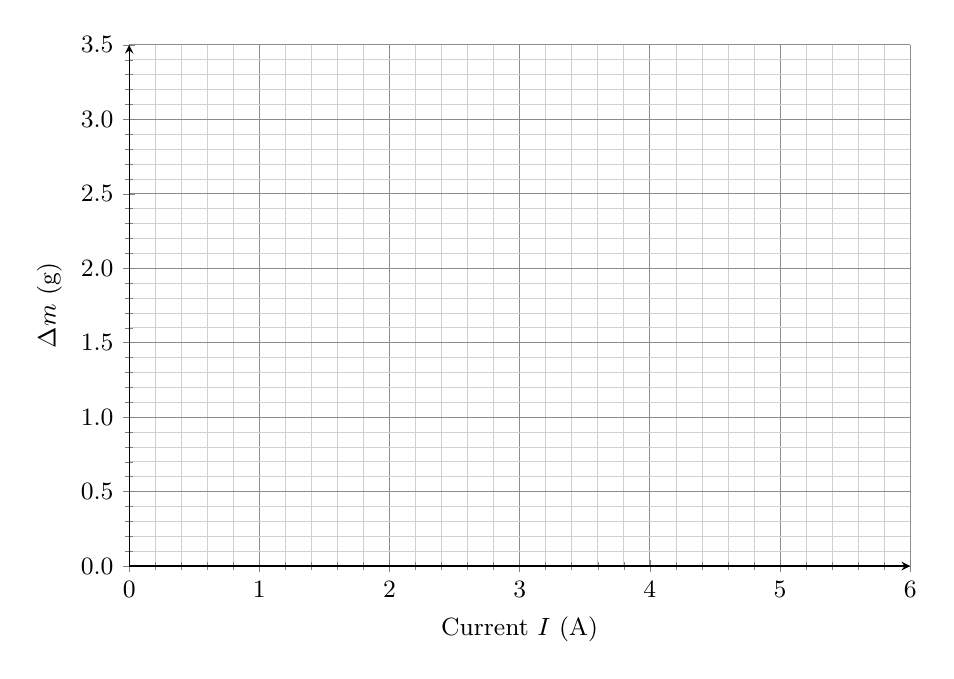
\begin{tikzpicture}
    \begin{axis}[width=115mm, height=82mm, axis lines=left, xmin=0, xmax=6, ymin=0, ymax=3.5,
        xtick={0,1,...,6}, ytick={0,0.5,...,3.5}, minor x tick num=4, minor y tick num=4,
        grid=both, major grid style={black!45, line width=0.35pt}, minor grid style={black!18, line width=0.25pt},
        tick label style={font=\small}, label style={font=\small},
        yticklabel style={/pgf/number format/fixed, /pgf/number format/fixed zerofill, /pgf/number format/precision=1},
        xlabel={Current $I$ (\si{A})}, ylabel={$\Delta m$ (\si{g})},
        scaled ticks=false, enlargelimits=false]
      \addplot[draw=none] coordinates {(0,0)};
    \end{axis}
  \end{tikzpicture}
\end{center}
\qpartL{c}{2}{Use your graph to determine the strength of the magnetic field.}{5}
\end{saq}

% ---- Q9 (rod held up by the motor effect)
\Needspace{30\baselineskip}
\begin{saq}{4}
A horizontal copper rod of mass \qty{30}{g} and length \qty{0.20}{m} hangs from two light, flexible
leads. It is in a uniform horizontal magnetic field of \qty{0.50}{T}, directed into the page.
\begin{center}
  \begin{tikzpicture}
    \fill[black!5] (-0.6,-0.6) rectangle (4.6,1.6); \fieldin{-0.3}{-0.35}{4.3}{1.4}{0.5}
    \draw[line width=1pt] (0.3,2.4) -- (0.3,0.4); \draw[line width=1pt] (3.7,2.4) -- (3.7,0.4);
    \draw[line width=3pt] (0.3,0.4) -- (3.7,0.4); \node[right, font=\small] at (4.7,0.4) {rod}; \draw[line width=0.3pt] (3.75,0.4) -- (4.7,0.4);
    \fill[pattern=north east lines] (-0.2,2.4) rectangle (4.2,2.6); \draw (-0.2,2.4) -- (4.2,2.4);
  \end{tikzpicture}
\end{center}
\qpartL{a}{2}{Calculate the current needed in the rod for the tension in the leads to be zero.}{5}
\qpartL{b}{1}{State the direction of this current in the rod.}{2}
\qpartL{c}{1}{Describe the motion of the rod if this current is doubled.}{2}
\end{saq}

% ---- Q10 (force between the wires of a cable)
\Needspace{22\baselineskip}
\begin{saq}{3}
A power cable has two long parallel conductors \qty{3.0}{mm} apart. They carry a current of \qty{10}{A}
to and from an appliance.
\qpartL{a}{2}{Calculate the force per metre between the conductors, and state whether it is attractive
or repulsive.}{5}
\qpartL{b}{1}{Describe how this force changes if the current in the cable is doubled.}{2}
\end{saq}

% =====================================================================
\topictitle{Topic 3 - Electromagnetic Induction}

% ---- Q11 (Faraday's law calculation)
\begin{saq}{4}
A square coil of 50 turns, each of side \qty{8.0}{cm}, is at right angles to a uniform magnetic field.
The field increases steadily from \qty{0.20}{T} to \qty{0.80}{T} in \qty{0.30}{s}. The coil has a
resistance of \qty{4.0}{\ohm}.
\qpartL{a}{1}{Calculate the change in magnetic flux through one turn of the coil.}{3}
\qpartL{b}{2}{Calculate the average emf induced in the coil.}{4}
\qpartL{c}{1}{Calculate the average current in the coil.}{2}
\end{saq}

% ---- Q12 (magnet dropped through a coil)
\Needspace{40\baselineskip}
\begin{saq}{4}
A bar magnet is dropped, north pole first, through a vertical coil connected to a data logger, which
records the emf in the coil.
\begin{center}
  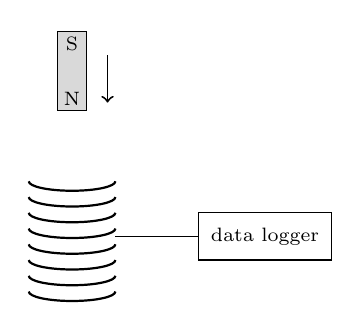
\begin{tikzpicture}
    \draw[fill=black!15] (-0.18,2.6) rectangle (0.18,3.6); \node[font=\scriptsize] at (0,2.75) {N}; \node[font=\scriptsize] at (0,3.45) {S};
    \draw[->, line width=0.7pt] (0.45,3.3) -- (0.45,2.7);
    \foreach \y in {0.3,0.5,...,1.7} \draw[line width=0.8pt] (-0.55,\y) arc (180:360:0.55 and 0.12);
    \draw (0.55,1.0) -- (1.6,1.0); \draw (1.6,0.7) rectangle (3.3,1.3); \node[font=\scriptsize] at (2.45,1.0) {data logger};
  \end{tikzpicture}\hspace{12mm}%
  \begin{tikzpicture}
    \draw[axisline] (0,0) -- (5.2,0) node[right] {$t$};
    \draw[axisline] (0,-1.8) -- (0,1.9) node[above] {emf};
    \node[left, font=\small] at (0,0) {0};
  \end{tikzpicture}
\end{center}
On the axes, sketch the emf against time as the magnet falls through the coil, and explain the main
features of your graph.
\alines{8}
\end{saq}

% ---- Q13 (transformer)
\Needspace{30\baselineskip}
\begin{saq}{5}
A transformer converts \qty{240}{V} AC to \qty{12}{V} AC to supply a \qty{12}{V} lamp that draws
\qty{6.0}{A}.
\qpartL{a}{1}{Calculate the turns ratio $N_\mathrm{p} : N_\mathrm{s}$.}{2}
\qpartL{b}{2}{Assuming the transformer is ideal, calculate the current in the primary coil.}{4}
\qpartL{c}{2}{The real transformer is 90\% efficient. Calculate the current in its primary coil.}{4}
\end{saq}

% ---- Q14 (energy losses in real transformers)
\Needspace{110mm}
\begin{saq}{4}
Explain TWO reasons why a real transformer is less than 100\% efficient, and describe a way of reducing
each energy loss.
\alines{10}
\end{saq}

% ---- Q15 (transmission losses)
\Needspace{30\baselineskip}
\begin{saq}{5}
A small power station transmits \qty{200}{kW} to a town through transmission lines of total resistance
\qty{0.50}{\ohm}.
\qpartL{a}{3}{Calculate the power lost in the lines if the energy is transmitted at \qty{2.0}{kV}, and
if it is transmitted at \qty{20}{kV}.}{7}
\qpartL{b}{2}{Explain why transformers are needed at both ends of a transmission line.}{4}
\end{saq}

% =====================================================================
\topictitle{Topic 4 - Applications of the Motor Effect}

% ---- Q16 (DC motor torque)
\begin{saq}{5}
The rectangular coil of a DC motor has 200 turns and measures \qty{5.0}{cm} by \qty{4.0}{cm}. It carries
a current of \qty{1.5}{A} in a uniform magnetic field of \qty{0.35}{T}.
\qpartL{a}{2}{Calculate the maximum torque on the coil.}{4}
\qpartL{b}{3}{Explain why the torque on the coil changes as the coil rotates, and why a split-ring
commutator is needed for the motor to keep turning in one direction.}{7}
\end{saq}

% ---- Q17 (back emf)
\Needspace{26\baselineskip}
\begin{saq}{5}
A DC motor is connected to a \qty{12}{V} supply. The resistance of its coil is \qty{1.5}{\ohm}.
\qpartL{a}{1}{Calculate the current in the motor at the instant it is switched on.}{2}
\qpartL{b}{2}{When the motor is running at full speed, the current is \qty{1.2}{A}. Calculate the back emf.}{4}
\qpartL{c}{2}{Explain why a motor can overheat and burn out if it is jammed so that it cannot turn.}{4}
\end{saq}

% ---- Q18 (AC and DC generators)
\Needspace{110mm}
\begin{saq}{4}
Compare the structure and the output of a simple AC generator with those of a simple DC generator.
\alines{10}
\end{saq}

% ---- Q19 (AC induction motor)
\Needspace{110mm}
\begin{saq}{4}
Explain how an AC induction motor produces a torque on its rotor.
\alines{10}
\end{saq}

% ---- Q20 (magnetic braking: Lenz's law and energy)
\Needspace{30\baselineskip}
\begin{saq}{5}
On some roller coasters, copper fins on the cars pass between strong permanent magnets near the end of
the ride, which slows the cars down without any contact.

Analyse how this braking system works. In your answer, refer to Lenz's law and the law of conservation
of energy, and explain why the braking force decreases as the cars slow down.
\alines{12}
\end{saq}

\end{document}
